\subsection{Robustheit gegenüber Lichtverhältnisse}
\label{sec:brightness_eval}
\subfigbox{
\subfigure[Offset]{\label{subfig:brightness_offset}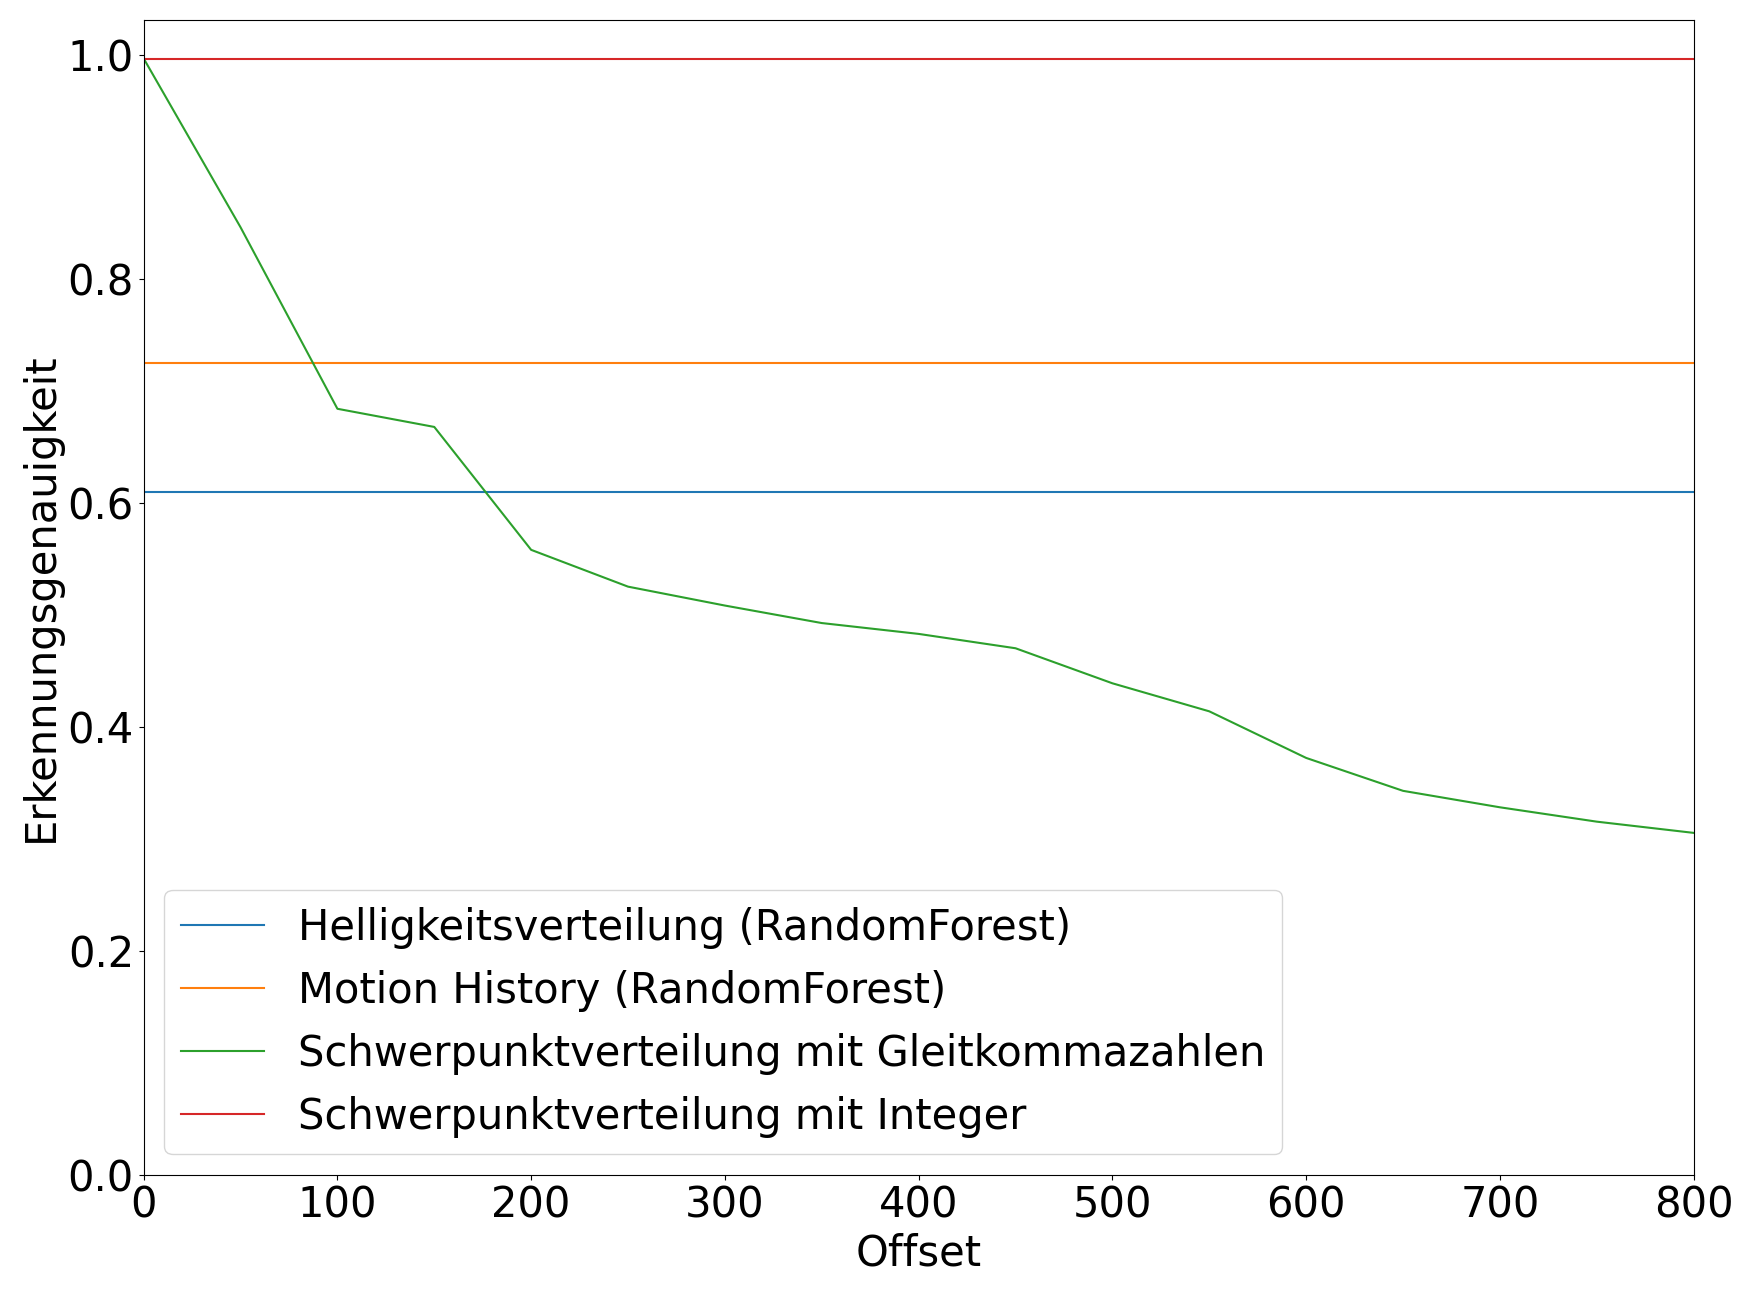
\includegraphics[width=0.495\linewidth]{images/brightness_offset.png}}\hfill%
\subfigure[Skalierung]{\label{subfig:brightness_scaling}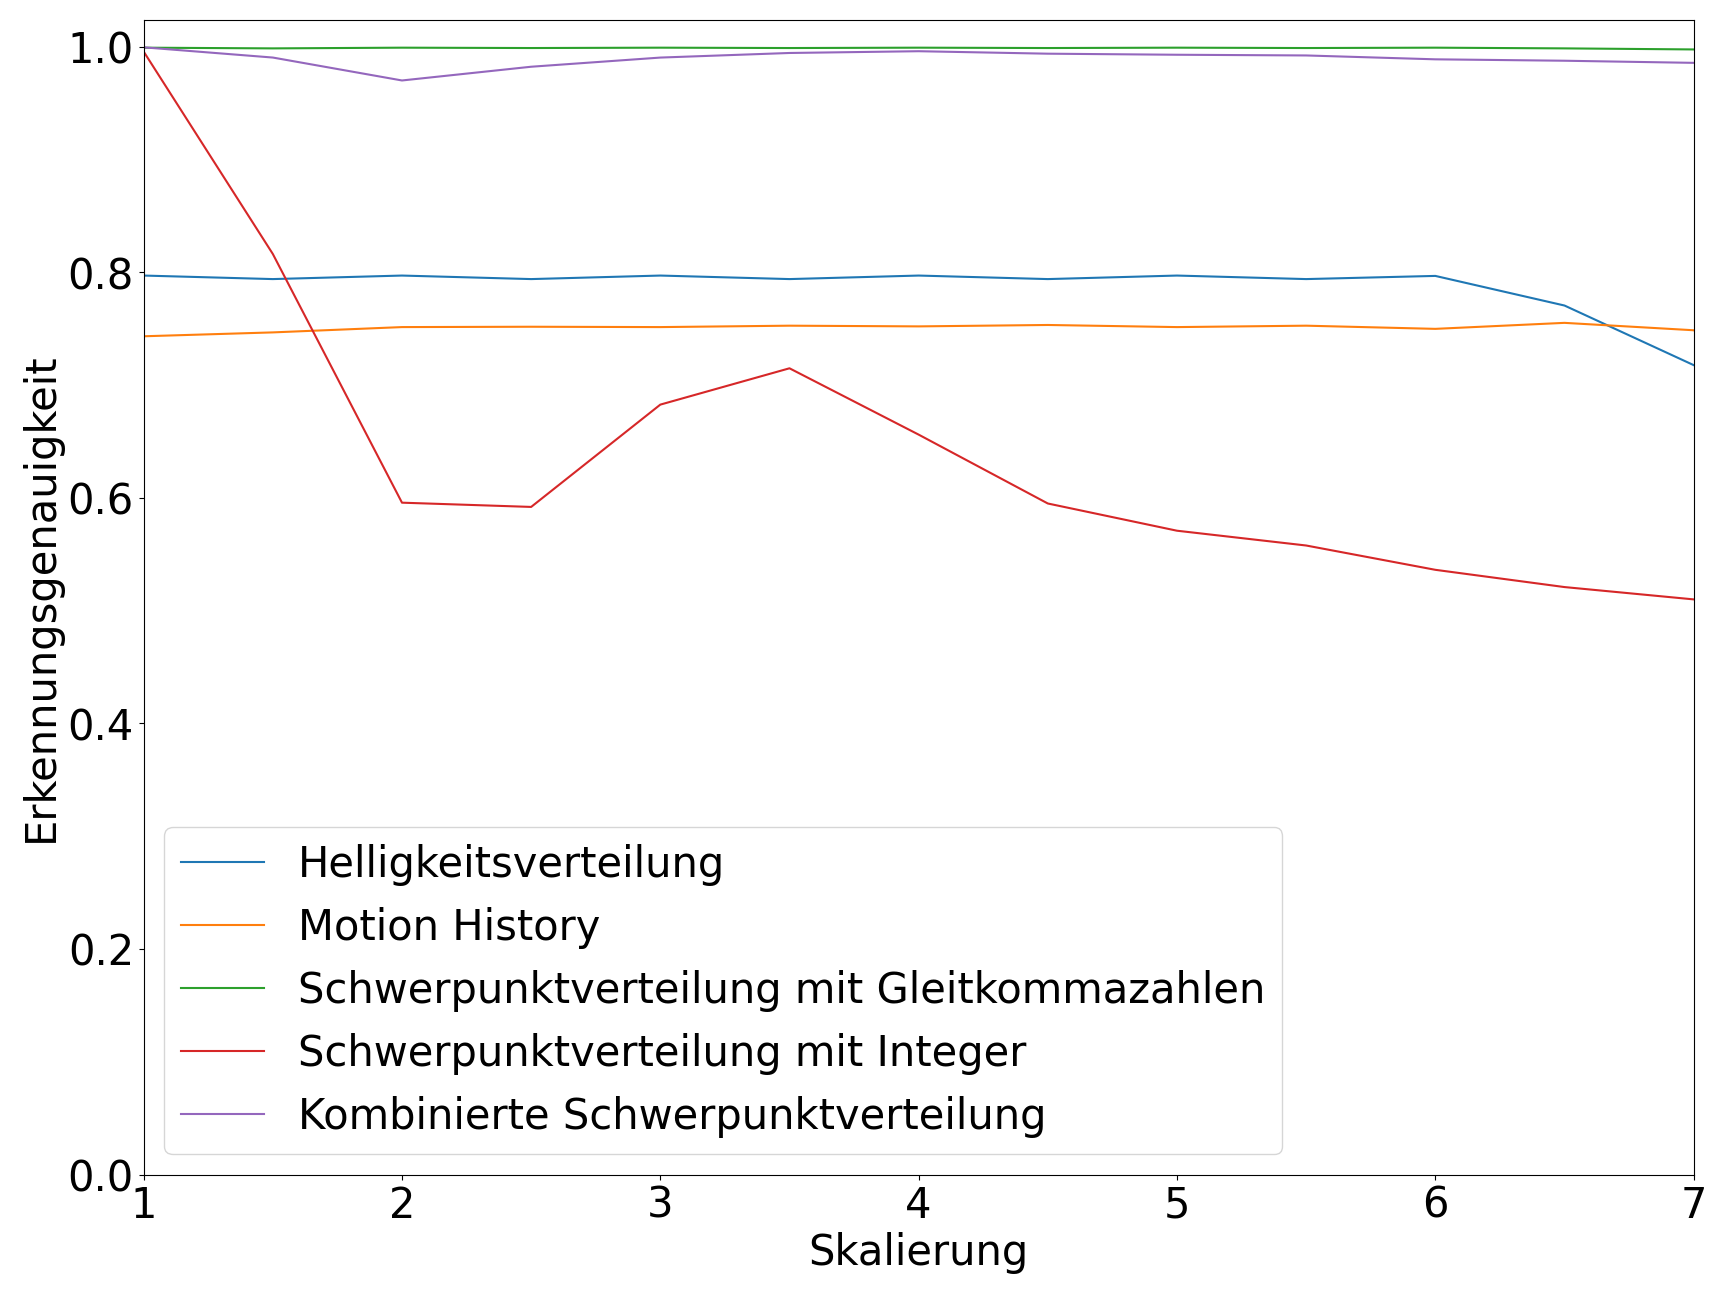
\includegraphics[width=0.495\linewidth]{images/brightness_scaling.png}}%
}{Ergebnisse der Helligkeitstestmenge 1 je Ansatz.}{fig:brightness}
In Sektion \ref{sec:DymelData} wurde die Helligkeitstestmenge 1 vorgestellt. Diese Testmenge modifiziert einen bestehenden Datensatz aus der Gestentestmenge indem Offset hinzugefügt
oder die Helligkeiten skaliert werden. Bei dem Offset verändert sich der Kontrast nicht, aber die Gesamthelligkeit steigt. Bei der Skalierung steigt die Gesamthelligkeit und der Kontrast wird stärker. Mit
dieser Testmenge sollen die Invarianzen der einzelnen Ansätze bewertet werden. Für die Helligkeitsverteilung und Motion History wurden die Konfigurationen gewählt, die insgesamt am besten waren, da die
Helligkeitstestmenge 1 auf der Gestentestmenge basiert.
\newline
\newline
Abbildung \ref{subfig:brightness_offset} zeigt, dass die Helligkeitsverteilung, Motion History und die Schwerpunktverteilung
mit Integer invariant gegenüber einen offset sind, wohingegen die Schwerpunktverteilung mit Gleitkommazahlen starke Defiziete aufweist.
Die kombinerte Schwerpunktverteilung ist nicht invariant und hat mit zunehmenden Offset eine schlechtere Erkennungsgenauigkeit.
\newline
\newline
Abbildung \ref{subfig:brightness_scaling} zeigt, dass die Schwerpunktverteilung mit Gleitkommazahlen invariant gegenüber Skalierung ist. Die Helligkeitsverteilung und Motion History weisen weitesgehend
keine Defiziete auf. Die Helligkeitsverteilung schwankt zwischen 6.5 und 7, allerdings findet ab dieser Skalierung der resultierende Wert bereits so groß, dass er teilweise auf den Maximalwert 1023
gesetzt wird. Die Schwerpunktverteilung mit Integer ist nicht invariant. Die kombinierte Schwerpunktverteilung weist keine Invarianz auf. Die Erkennungsgenauigkeit sinkt mit zunehmender Skalierung.
Insgesamt verhalten sich alle Ansätze wie erwartet.
\begin{figure}[h!]
    \centering
    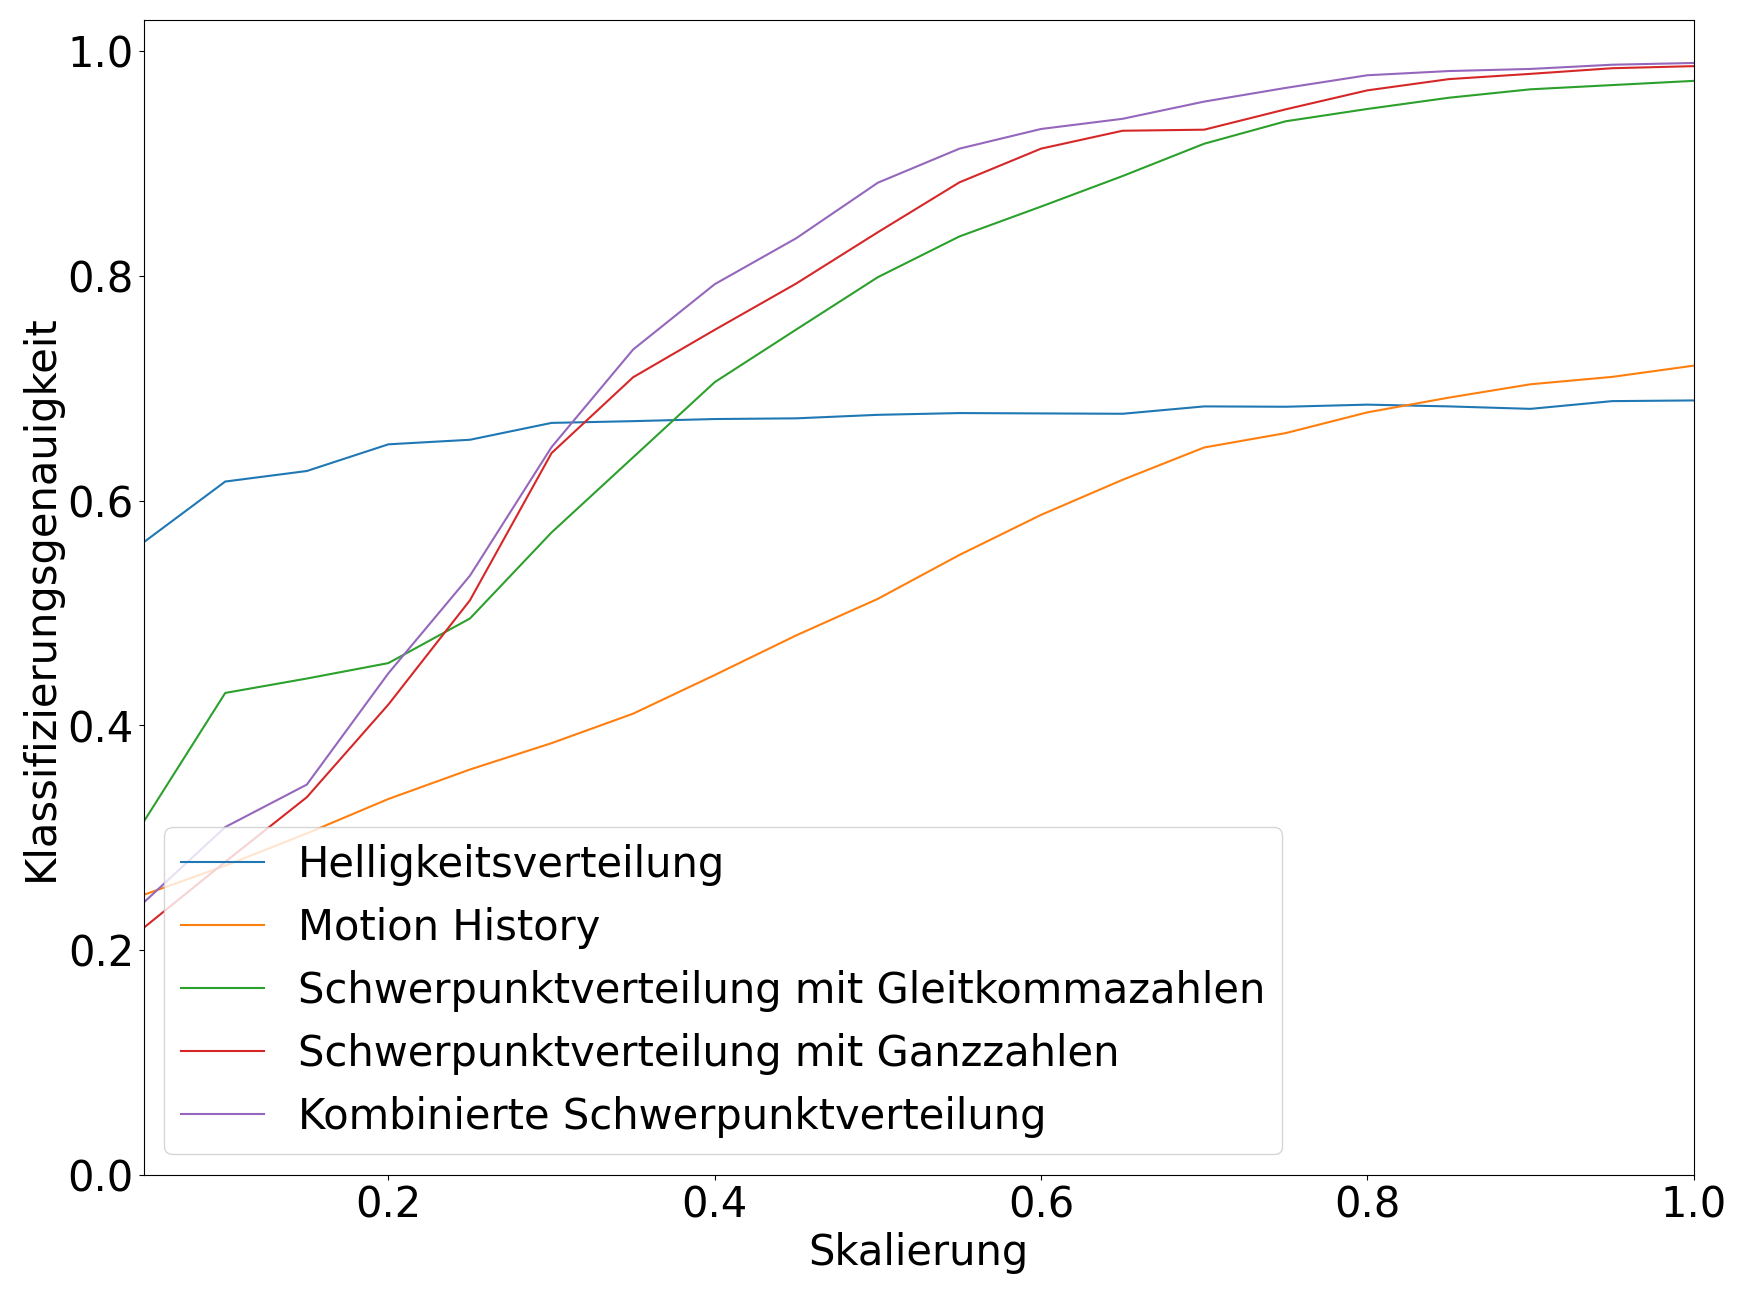
\includegraphics[width=\linewidth]{images/brightness2_scaling.png}
    \caption{Ergebnisse der Helligkeitstestmenge 2 je Ansatz.}
    \label{fig:brightness2_scaling}
\end{figure}
\newline
\newline
Die Helligkeitstestmege 2 ist eine Mischung zwischen Skalierung und Offset. Die Gesamthelligkeit bleibt erhalten und der Kontrast zwischen dunklen
und hellen Pixeln verringert sich. Diese Situation ist vergleichbar mit einer zunehmenden Distanz zur Kamera, da dort der Kontrast durch Streulicht auch geringer wird.
\newline
\newline
Abbildung \ref{fig:brightness2_scaling} zeigt, dass ausschließlich die Helligkeitsverteilung eine Invarianz aufweist. Sie zeigt zwar auch auch Defiziete zwischen $0.05$ und $0,3$ auf, aber in diesem
Intervall ist der Kontrast bereits sehr gering. Die Schwerpunktverteilungen verhalten sich der Erwartung gemäß, da keine invariant gegenüber Offset und Skalierung ist. Entgegen der Erwartung verhält
sich die Motion History.
\newline
\newline
Abschließend ist die Helligkeitsverteilung am robustesten gegenüber die Lichtverhältnisse. Trotzdem erweisen sich die Schwerpunktverteilungen am besten, da die Erkennungsgenauigkeit deutlich höher ist
in den meisten Fällen.